\documentclass[../main.tex]{subfiles}
\begin{document}
\begin{enumerate}
    \item Selon vous, quelles figures parmi les suivantes sont des
    \textbf{quadrilatères} ?
    \vspace{1cm}
    \begin{center}\def\c{.45\linewidth}
    \begin{tabular}{p{\c}p{\c}}
    (a)
    \begin{center}
        \begin{tikzpicture}[scale=0.8]
            \coordinate(A)at(0,0);{\tiny }
            \coordinate(B)at(3,0);
            \coordinate(C)at(4,2);
            \coordinate(D)at(2.5,4);
            \coordinate(E)at(0,1.5);
            \draw(A)--(B)--(C)--(D)--(E)--cycle;
        \end{tikzpicture}
    \end{center}
    &(b)
    \begin{center}
        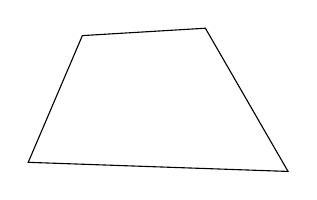
\begin{tikzpicture}[scale=0.7, rotate=120]
            \coordinate(A)at(0,0);{\tiny }
            \coordinate(B)at(3,0);
            \coordinate(C)at(4,2);
            \coordinate(D)at(2.5,4);
            \draw(A)--(B)--(C)--(D)--cycle;
        \end{tikzpicture}
    \end{center}
    \\(c)
    \begin{center}
        \begin{tikzpicture}[scale=0.7, rotate=120]
            \draw(0,0)circle(2);
        \end{tikzpicture}
    \end{center}
    &(d)
    \begin{center}
        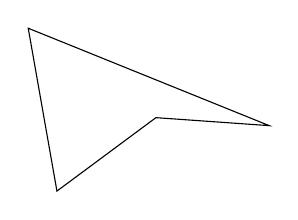
\begin{tikzpicture}[scale=0.7, rotate=-80]
            \coordinate(A)at(0,0);{\tiny }
            \coordinate(B)at(3,0);
            \coordinate(C)at(2,2);
            \coordinate(D)at(2.5,4);
            \draw(A)--(B)--(C)--(D)--cycle;
        \end{tikzpicture}
    \end{center}
    \end{tabular}
    \end{center}
    \item Écrire la \textbf{définition d'un quadrilatère.}
    \end{enumerate}
\end{document}